\documentclass[a4paper]{article}
\usepackage[utf8]{inputenc}
\usepackage{graphicx}
\usepackage[section]{placeins}

\usepackage[
	citestyle=ieee, 
    bibstyle=ieee,
    style=numeric-comp,
]{biblatex}
    
\addbibresource{ref.bib}


\title{The Necessity of Microservices in a DevOps Environment}
\author{
{Julius Celik}\\
\textit{
    jcelik@kth.se
} \and {Patric Ridell}\\
\textit{
    pridell@kth.se
}}
\date{\today{}}

\setlength{\parindent}{0em}
\setlength{\parskip}{1em}

\begin{document}

\maketitle

% 10 Tech Challenges That Are Solved by Microservices
% https://medium.com/containerum/10-tech-challenges-that-are-solved-by-microservices-d91adeecb2e7

\section{Introduction}
Microservices is a software development method where systems are divided into smaller parts, called microservices, that can be individually deployed. In turn, this enables low coupling, high cohesion, and strong composibility. The microservices are focused on performing single tasks really well, and implementing functionality by composing multiple microservices. It also enables multiple developers to work on a common codebase while minimizing obstruction, which becomes more notable in larger systems, with a greater number of developers.

The opposite of microservices are often called monoliths. A monolith is a whole system implemented as a single application. This means that the system is always handled as a single entity, which in practice means that the whole system has to be running to perform integration tests on parts of the system, and the whole application is duplicated when the system is scaled in a distributed manner.

Microservices developed as a natural response to agile organizational structures. Agile development has become the industry norm for software development \cite{Jeremiah}. Within agile development, companies organize their software developers in smaller teams of usually four to eight developers, where the teams have full life cycle ownership of the software they write. This shift toward agile working environments along with a system archtecture based on microservices can be summarized by Conway's law, which states that:
\begin{quote}
    Any organization that designs a system (defined broadly) will produce a design whose structure is a copy of the organization's communication structure. \cite{Conway}
\end{quote}

As organizations divide software developers into self managed teams, Conway's law implies that it is a natural progression to divide the systems into decoupled services that can be independently deployed, as to mirror the organization's communication structure.

An organizational structure that allows a small team of developers to work with full life cycle ownership of their product, will also open up opportunities for shorter software iterations. This is closely related to the use of DevOps. DevOps is a set of processes that integrate and combine cultural philosophies, practices and tools that allow an organization to deliver more reliable software at a faster rate than traditional software development \cite{aws}. As we will see throughout this paper, the combination of microservices and DevOps will create a highly competitive environment for software development.

% The problem with monoliths
% https://smartbear.com/solutions/microservices/

\section{Benefits of microservices within DevOps}
\label{sec:benefits}
% The difficulties of using a CI on a large monolith. Every change triggers a rebuild/retest of everything
In a monolith application, there is an ever increasing difficulty for \textit{Continuous Integration} (CI). With every small modification of the codebase, one might have to build and deploy an entire new version of the application \cite{Jeremiah}. This section will explore how microservices tackle this problem and in what ways they enable CI, a foundation of DevOps. We will see that in most cases, DevOps and microservices go hand-in-hand and augment each others functionality.

\subsection{Microservices enable individual deployments}
% All or nothing deployments. Individual deployments
At the core of microservices is modularity; doing one specific task really well. A consequence of the modular nature of microservices is the possibility of individual deployments. For some developers like \citeauthor{Newman2015} the ability to individually deploy microservices is even one of the fundamental definitions of microservices \cite{Newman2015}. The importance of this defining trait will be clear if we view it from the perspective of a larger system.

When a system becomes so large that multiple teams of developers work on it, changes to the system are done very frequently. If the teams use agile methods like CI the work done by every developer should be merged into a shared repository multiple times a day. With many people working on the same application that becomes hundreds or thousands of merges every day. At a certain point it becomes impossible for every change to trigger a new run of the CI-pipeline, as the CI would be overloaded where multiple new updates comes as the CI executes a single run. This leads to multiple problems when deploying releases.

\subsubsection{Avoiding large-impact and high-risk deployments}
The difficulty of releasing a monolith is based on multiple problems. One problem is that the deployments become larger and therefore take longer time. Additionally, and maybe more importantly, it becomes more difficult to deploy a large monolith compared to a microservice. \citeauthor{Newman2015} highlights the potential for such a deployment to be \textit{large-impact} and \textit{high-risk}. \citeauthor{Newman2015} claims that this leads to deployments happening infrequently due to understandable fear. This leads to larger changes between releases, which develops a higher risk for something wrong to be released. \cite[p.~6]{Newman2015}

Infrequent deployments lead to larger software-deltas and longer feedback loops. When something wrong happens it is difficult to understand why it is wrong because it might have been a long time since the change was implemented, and there might be many changes since the last release. This behaviour will impact the quality and speed of the whole development cycle and make it difficult to create an effective DevOps environment. With microservices we can instead produce more frequent \textit{low-impact} and \textit{low-risk} deployments for a more sustainable and dependable development cycle.

\subsubsection{Fault management and automation}
Another problem that is related to releasing monoliths is the ability to use rollbacks, and the use of \textit{Continuous Deployment} (CD). For the reasons mentioned above it is difficult and often impossible to use CD, and when a faulty system is released, it is often difficult to rollback the system to a previous stable version.

With microservices it is easy to release every minor update of the service, and to release often. It is therefore very easy to automate releases with CD's as well as managing releases with canary releases, where the update is only deployed on a small percentage of the servers, or exposed to a small percentage of users, and predefined metrics are verified to be sufficient before deploying the change to all of the servers. Canary releases require a measurable goal to be defined, like all requests to a service should be responded to within 500ms. With a microservice one or a few metrics can be defined and measured for every microservice. For a monolith that would require a very large amount of metrics to be measured, which would be difficult to both maintain and measure.


\subsection{Quicker feedback loops with fine grained modular testing}
% Quicker testing of parts of system. Feedback loop.
Decreasing the time between the releases of new features is a highly valuable trait within the DevOps development cycle. Microservices enable this through quicker feedback loops that allow testing of smaller and more specific parts of the system. When testing a monolith, no separate parts of the application can be mocked, which means that even to test a part of the system, the whole system has to be running. This leads to large overhead for smaller integration tests, and also difficulties in performing service and integration tests on parts of the system. Within DevOps, this obstructs the use of automatic testing which is crucial for an effective DevOps implementation. 

Another benefit of microservices, is that parts of the system can be tested together, without the whole system running. It is crucial to perform service and integration tests, to maintain high quality software. It is also important for establishing a good feedback loop, which is fundamental to DevOps.

\subsection{Automatic and independent scalability}
% Automatic scalability
The architecture used within an application can either work as a bottleneck on the growth of the application or be a tool that enables expansion. Although it is certainly possible to maintain a large monolith system, there are definitely easier and more effective ways. To scale a monolith service, every part of it has to be scaled simultaneously \cite{Newman2015}. Microservices allows a developer to prepare for future expansion by making the architecture more scalable. A developer can scale a specific service where it is needed, while leaving others unchanged \cite{Newman2015}.

Automatically scaling the infrastructure is a common DevOps practice which can ensure that resources are available when user demand is high, at the same time as ensuring that you do not overpay for infrastructure \cite{Pinedo2015}. For automatically scaling of infrastructure to work, there has to exist measurable metrics like resource-usage, response time, event-queue length, or dropped packages. With microservices it is very easy to define these metrics as a microservice often only does one thing. Therefore it is clear that you measure how well the service does that one thing. With a monolith it is a lot more difficult to define a good metric as a monolith does a lot of different things, and defining a scaling strategy becomes very complicated.

It is also difficult to predict and profile a monolith to understand what part of the system is underperforming or gets unevenly loaded. With microservices it is easy to monitor service load, and performance. The clearly defined system boundaries offer an easy way to profile the system, which simplifies scalability decisions.

\subsection{Decoupling team dependencies}
\label{sec:benefits:team-dependencies}
When developing a monolith system there is always a risk that coupling creeps into the codebase by multiple modules using the same database tables, business logic being implemented in shared libraries, or implementations not being abstracted enough. When a team wants to change a part of the code that has multiple dependants in code maintained by other teams, it requires that the different teams coordinate. These coordinated efforts can take months to implement, as it often requires multiple people to discuss the changes over multiple meetings. This is a task that can not be solved with automation which would be the desirable DevOps solution.

Of course coupling can appear in microservice systems both by multiple services using the same database tables, or business logic being implemented in shared libraries. It is however a lot easier to identify and avoid coupling in microservices. It is more explicit if multiple microservices depend on a shared library, than it is to understand that multiple parts of a single application depend on a shared piece of code. It is also very easy to avoid multiple microservices using the same databases as it is clearer to understand when only one microservice uses a database, versus only a distinguished part of an application uses a database. Coupling is also avoidable for monoliths, however it is not as easy, and large monolith systems are often very coupled.

With microservices and the concept of individual deployments these team dependency problems are largely avoided. This is why individual deployability is so fundamental to microservices. If a team wants to change the implementation of their microservice it does of course not affect any other teams, as one can be certain that other teams only depend on your microservices interface. If a team wants to update the interface of a microservice the team can deploy both an old version and a new version of the microservice, or just two interfaces to the same service. Other teams get to migrate to the new version of the updated service gradually. When all dependants have migrated to the new version of the microservice the old version can be removed. This is shown in figure \ref{fig:microservice-versioning}.

This migration method is only possible to accomplish with microservices, and completely eliminates the previous problems with team dependencies. This enables teams to move quicker and be less dependant of each other. It is a requirement for DevOps practices like CI and CD to be used.

\begin{figure}[h]
    \centering
    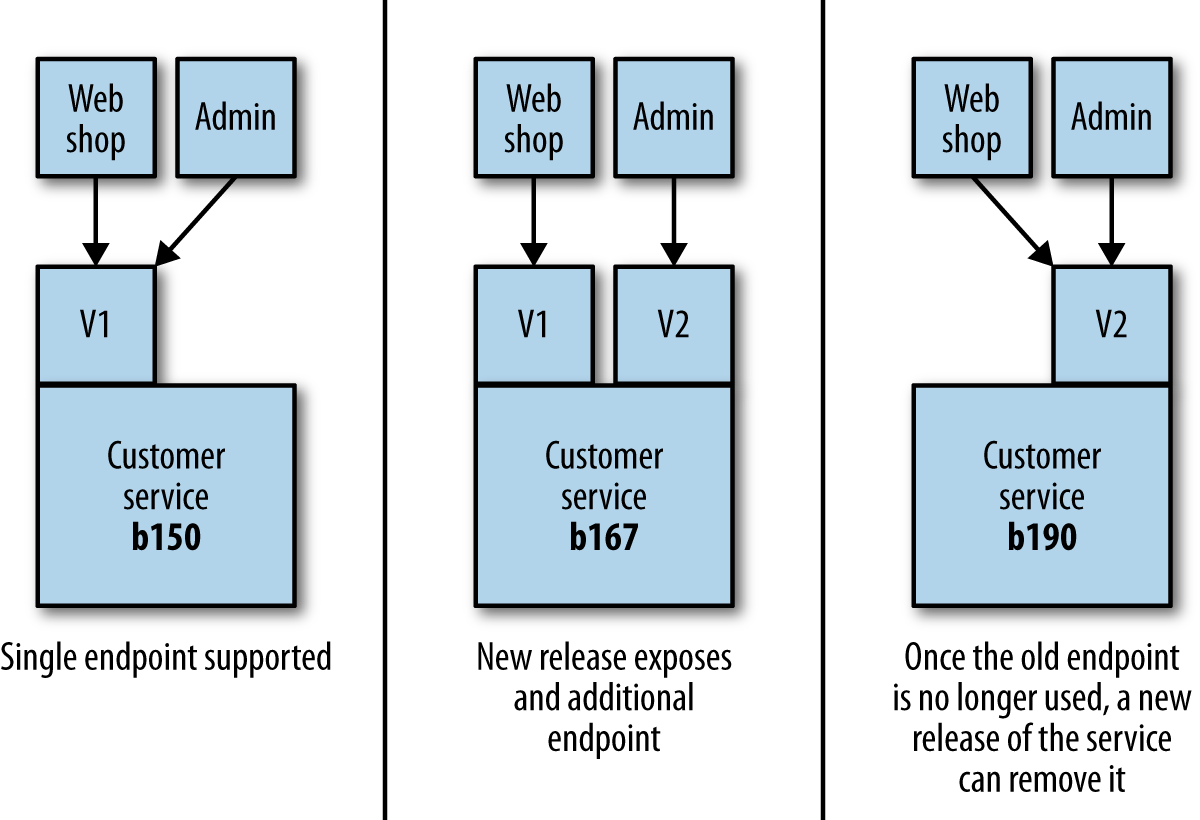
\includegraphics[width=\textwidth]{microservice-versioning.png}
    \caption{``\textit{Coexisting different endpoint versions allows consumers to migrate gradually}'', borrowed from \cite{Newman2015}}.
    \label{fig:microservice-versioning}
\end{figure}


\pagebreak
\section{Potential pitfalls}
\label{sec:pitfalls}
% https://blog.christianposta.com/microservices/when-not-to-do-microservices/

Up to this point we have focused on the benefits of using microservices. However, as with all tools, there are some aspects that a user should be aware of to be able to utilize the full potential of the tool and avoid misuse. In this section, we will discuss the consequences of using microservices, and if there are any circumstances under which microservices should not be used at all. The goal is to begin creating a roadmap to ensure that your experience with microservices will be as smooth as possible, enabling you to focus on delivering products with speed and reliability. This section will be focused on the general understanding of the pitfalls of microservices and not specifically to DevOps.


\subsection{Microservices comes with complexity}
\label{sec:pitfalls:complexity}
The infrastructure for a monolith can be very easy to maintain. It might be a single server with a database and an application running. By introducing microservices into that architecture a lot of problems have to be solved like, ``\textit{how are services communicating with each other}'', ``\textit{how are services discovered}'', ``\textit{how is state shared}'', and ``\textit{how is user authentication and authorization handled}''. When developing a monolith everything is in one place and it is easy to access any information necessary.

With more microservices, there is more surface area for security oversights to appear. Handling access control to different services could become a challenge in itself. If this is not done correctly and the wheel has to be reinvented for every microservice, mistakes will happen, leaving the system vulnerable for malicious attacks.

One of the most complicated challenges with microservices is defining system boundaries. It is not often that a developer or systems architect understand how a piece of software should function in detail, before beginning to develop it. The same is even worse for trying to fully understand the structure of a system. That is one of the most vital arguments for using agile software development methods instead of the waterfall method.

With microservices it is immensely painful to change the structure of the system, as there are a lot of distributed dependants. System changes are asynchronous, as services are independently released. That requires team wide synchronization on an immense level, which might not always be possible. This can be avoided by starting with a monolith architecture and letting the system gradually develop into a microservice architecture when it is a natural progression. This will ensure that the system is developed around clear bounded contexts and properly mirrors the business domain. \cite{Fowler2015}

\subsection{Bad patterns are magnified}

As previously discussed (section \ref{sec:benefits:team-dependencies}) coupling is a major problem that requires teams to coordinate releases, which can become a severe burden, leading to a long \textit{Time to Market} (TTM). It is a lot easier to avoid coupling when using microservices as a consequence of the nature of microservices. An area to look out for however is that if coupling appears, and teams have to synchronize releases, the problems related to coupling are magnified with orders of magnitude.

As microservices are independently and asynchronously released it is impossible to synchronize the release of two microservices. With a monolith a synchronized release can easily be implemented and tested to ensure that the team wide update works. With a microservice it can be a lot more difficult. The problem can be solved but no solution is perfect. The whole system could be taken down to release the multiple updates, but that can be disastrous for some businesses. The best solution is to eliminate the coupling over time, as a prerequisite for the update to take place. First when the update is contained to one microservice, the update can take place with version migration as explained in figure \ref{fig:microservice-versioning}.

\subsection{Using microservices to early}
Most of the benefits with microservices are only apparent when a lot of developers are working on the same system. If the development division is only one or two agile teams, microservices might not give any benefits, while it brings all the complexity that was discussed in section \ref{sec:pitfalls:complexity}. \citeauthor{Fowler2015}, \citeauthor{Newman2015} and \citeauthor{Buijze2018} among a lot of other experts emphasize the importance of starting out as a monolithic service, and then gradually splitting the monolith into microservices when the business domain and bounded contexts becomes more clear \cite{Fowler2015,Newman2015,Buijze2018}. \citeauthor{Fowler2015} has written a famous quote that is often referred to:
\begin{quote}
As I hear stories about teams using a microservices architecture, I've noticed a common pattern.
\begin{enumerate}
    \item Almost all the successful microservice stories have started with a monolith that got too big and was broken up.
    \item Almost all the cases where I've heard of a system that was built as a microservice system from scratch, it has ended up in serious trouble.\cite{Fowler2015}
\end{enumerate}

\end{quote}

As the system is new and small, with only a few developers working on it, it should be possible to use DevOps practices even though the system is a monolith. It is important to let the microservice system grow naturally. To help with deciding when to use microservices we include an infographic made by \citeauthor{Kerr} in figure \ref{fig:questions}.

\begin{figure}
    \centering
    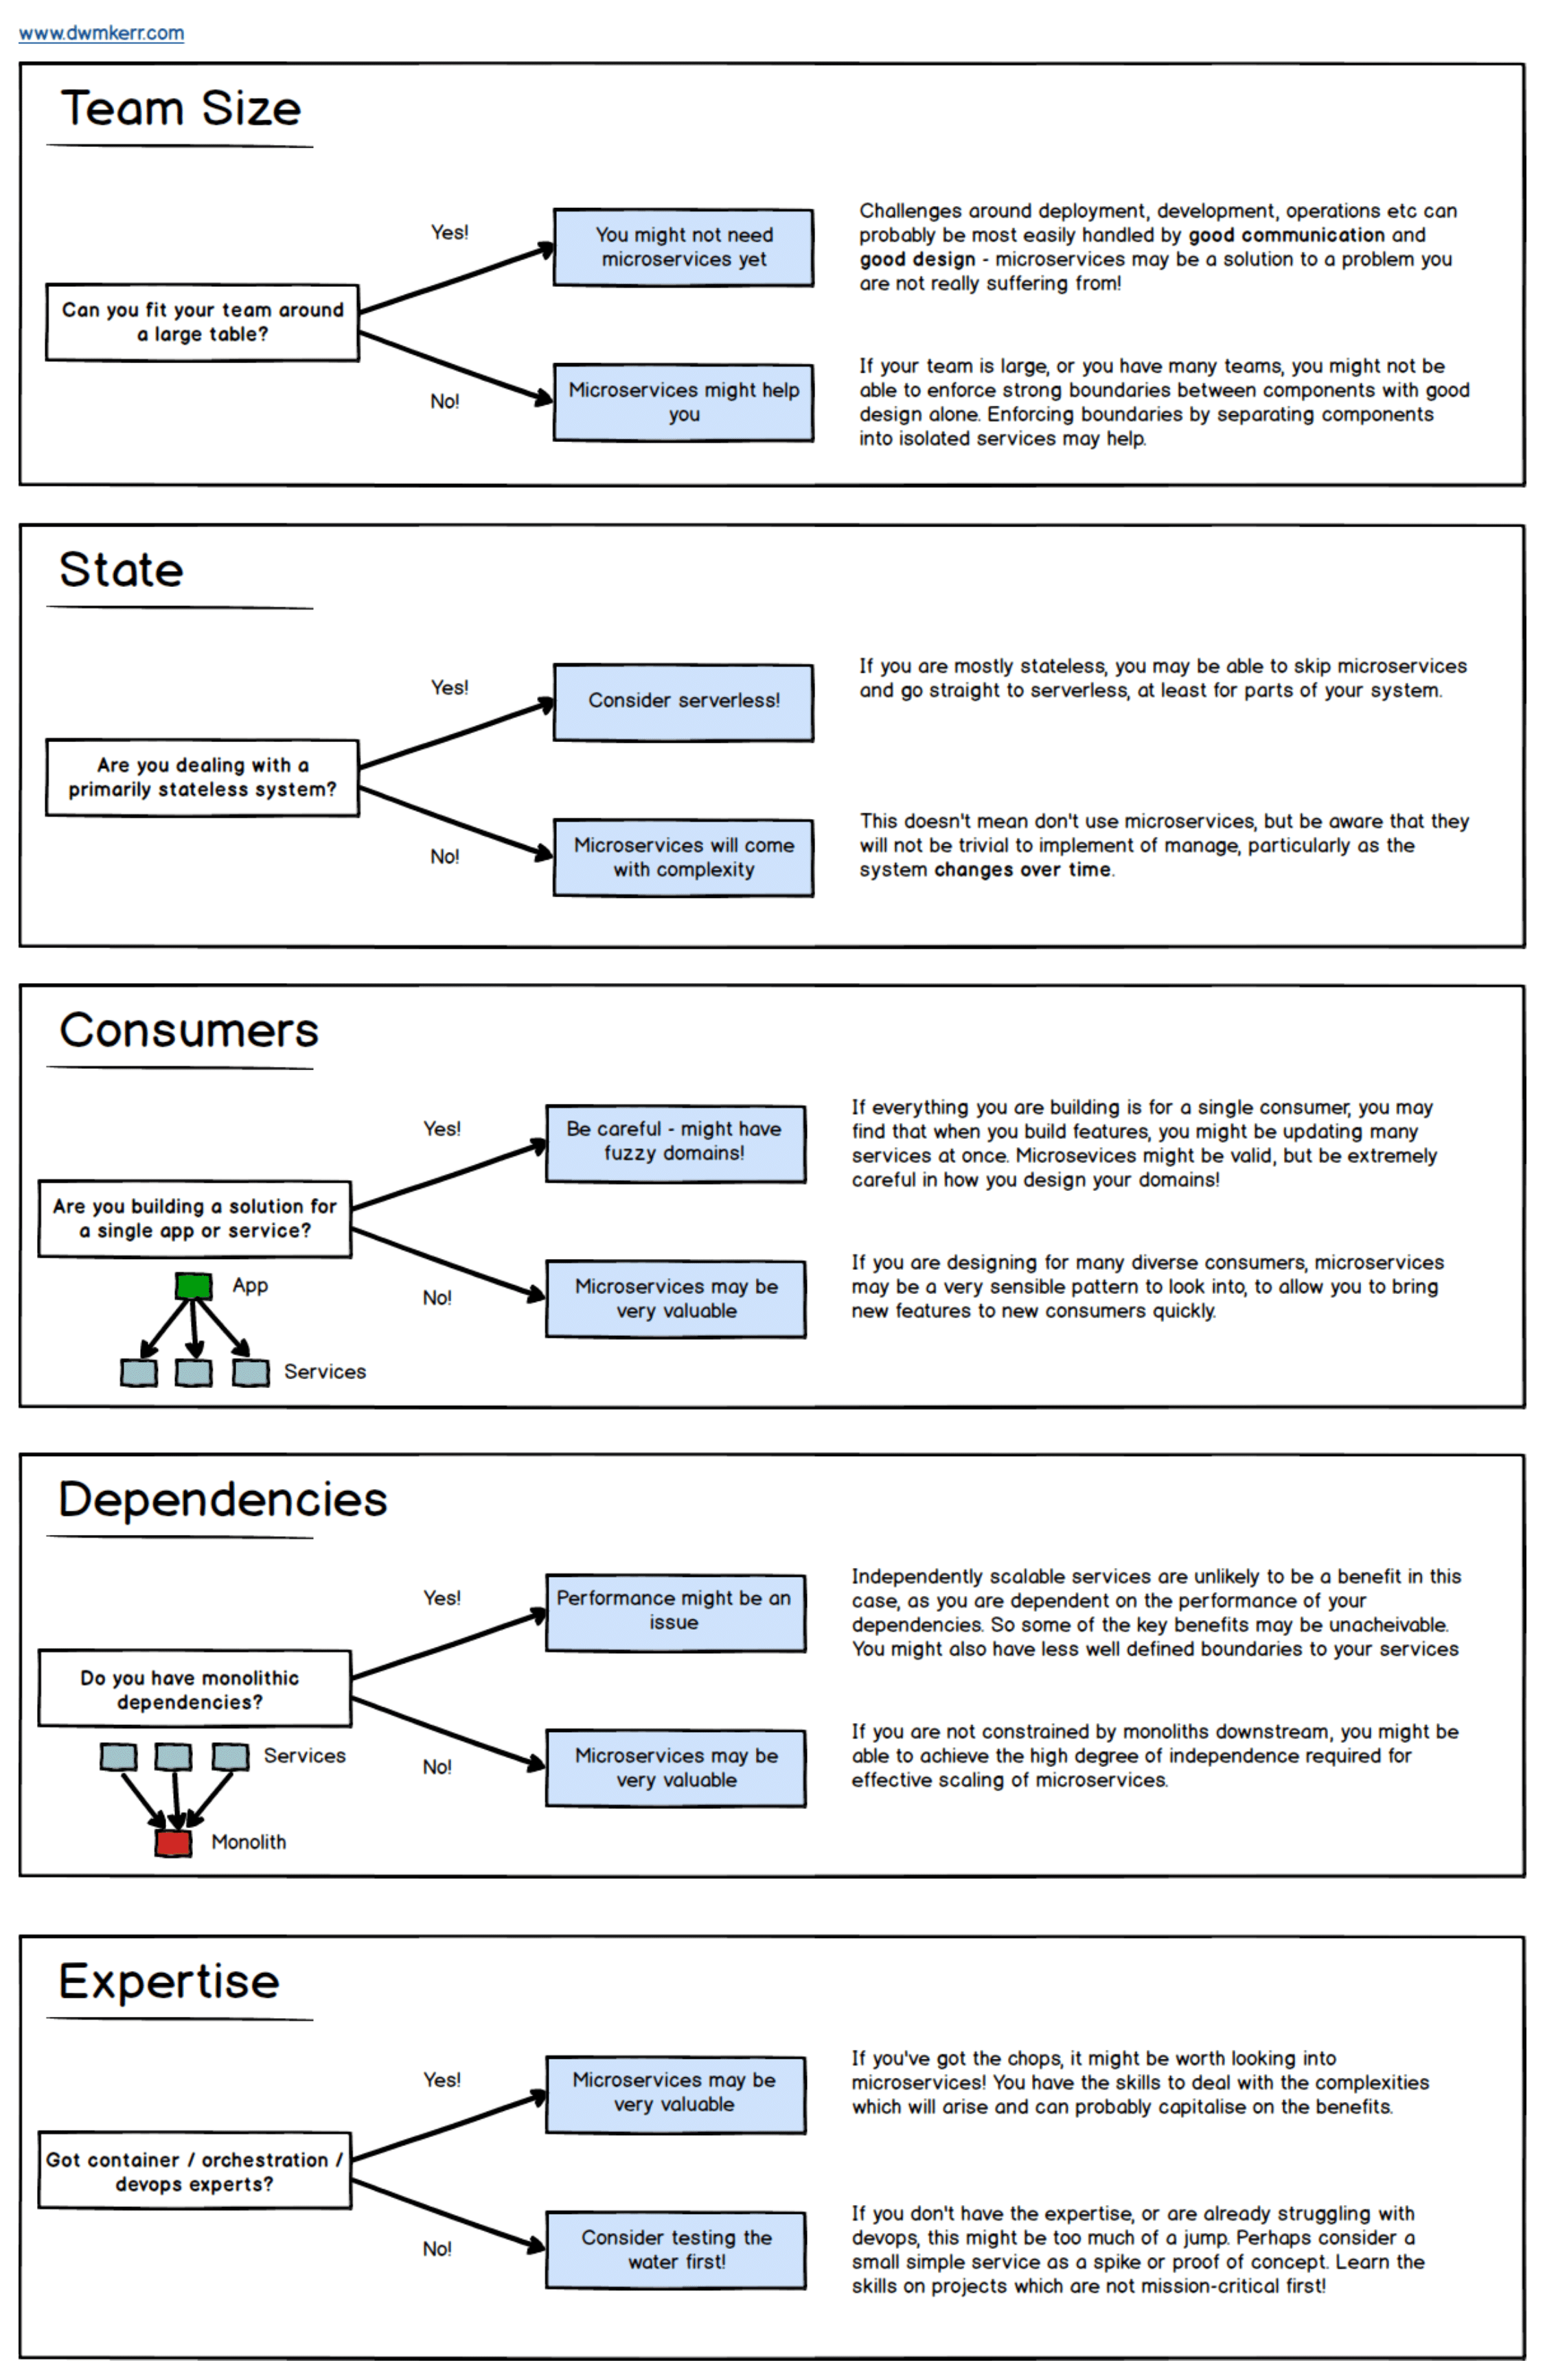
\includegraphics[width=0.95\textwidth]{microservice-questions.png}
    \caption{Infographic borrowed from ``\textit{The Death of Microservice Madness in 2018}'' \cite{Kerr}}.
    \label{fig:questions}
\end{figure}

\section{Conclusion}
This short essay only scratches the surface on why microservice are necessary when using DevOps practices. We introduced some concrete examples of why this is the case, as well as explained how to use microservices in practice together with DevOps. Some of the primary pitfalls of using microservices were also raised, so that if you do decide to use them, you will know how to use them correctly.

% Why microservices are essential to DevOps
Although there are some potential risks that a developer should be aware of when using microservices, they are far outweighed by the possibilities microservices bring. A major factor in staying competitive in any IT-related field is being \textit{first}. The early bird gets the worm. Being able to reduce time in-between iterations (and TTM) and quickly adapt to a changing business environment is essential for the longevity of all organizations. Using microservices in a DevOps environment will increase the likelihood of sustainable growth and at the same time increase competitiveness.


\newpage
\printbibliography

\end{document}
